%!TEX root = ../main.tex

\documentclass[../main.tex]{subfiles}
\begin{document}

\chapter{Introduction}
\label{chapter:introduction}

Our reliance on robots to keep our society functioning is increasing. With time, we find more and more applications where the use of robots is inevitable from the economical standpoint. Since the increase in robot usage drives the cost of the robot down, we should only expect more, better, smarter, and more reliable and cheaper robot in the future. A trend can be observed where if a task contains at least some amount of repetitiveness then this task will be automated in the near future. Most recently, the process of driving a car on the road or winning a game of Go, which was considered to be a human exclusive task, is already performed by computers equipped with some form of Artificial Intelligence. However, there are still a number of tasks that do not have automated solutions. These tasks vary from high impact tasks that directly impact lives to operations tasks that streamline operations of business and allow for products at a lower cost.

Some of these tasks include high impact tasks such as search and rescue in the wilderness, natural disaster monitoring and relief, demining, and surveillance. Other operation related tasks are floor sweeping, automated painting, field monitoring, and area scanning. All these tasks are different but they all share a common objective. In fact, in its most general form, these problems could be stated as a coverage path planning problem. An example of a robot performing a coverage task is shown in Figure~\ref{img:example_coverage}.

\begin{figure}[!hbt]
	\centering
	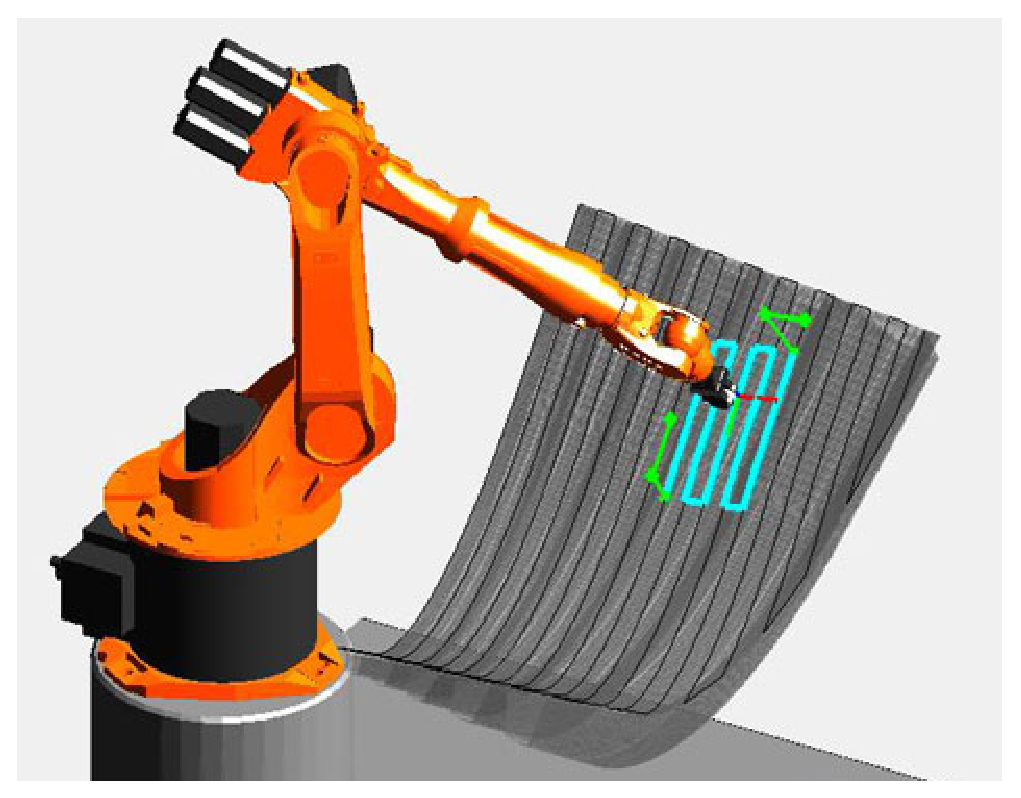
\includegraphics[scale=0.5]{img/chapter_1/example_coverage.eps}
	\caption{An example of an inspection coverage performed by a robotic arm.}
	\label{img:example_coverage}
\end{figure}

The coverage path planing problem is a problem of computing a path for a robot such that the traversal of that path by the robot results in all points in the environment being under the robot's footprint as some point of time during the traversal. The problem is as old as the machine controlled milling. Only in 2000, Arkin\cite{arkin2000approximation} has demonstrated that the problem is in fact NP-complete. As such, there are numerous approximate solutions that have been proposed over the years. There are two surveys by Choset~\cite{choset2000coverage} and Galceran~\cite{galceran2013survey} that outline the most accepted solutions. Moreover, there is an extension of this problem that has been gaining popularity over the recent years. The use of multi robot systems for coverage for better performance is becoming more appealing, motivated by the steady downwards trend of robot costs.

It is difficult to think about a good solution to the coverage path planning problem becomes the notion of \emph{goodness} varies from one application to another. For example, a good coverage path for a painting robot would results in the most uniform paint layer on the surface. A good coverage path for a monitoring application would result in the entire area recorded in high quality. Because of the variety of metrics, the existing solutions in the literature are typically very specialized. Other works in literature that focus on the theoretical analysis of the problem proposed solutions that theoretically achieve complete coverage but in practice, are not feasible for any robot with the simplest of dynamics.

In this work, we propose an approach that aims to make coverage paths more usable in practice. We do this by structuring the paths generated by our method to be as \emph{straight} as possible. This is motivated by the typical dynamics of robots. Straight line segments are the simplest path segments that a robot can traverse. Vast majority of robotic systems are designed in a way that travels between point $A$ and $B$ more efficiently in a straight line then any other way. In other words, we aim to compute paths with minimum number of turns. It should be noted that this goal can be achieved by minimizing the number of straight line segments requires for complete coverage since every straight line segment has a turn associated with it to transition to the next straight line segment.

Our main contributions in this work are several. First, we design our own metric called the altitude that aids with the computation of the number of lines for full coverage. We then propose a greedy algorithm that partitions the workspace into regions with the minimum overall altitude. The result of the algorithm is a workspace partition with a set of lines. One of the important aspects of the algorithm is the procedure to make a minimum altitude cut dividing a polygon into two. We then solve the coverage problem by planning a tour of straight line segments by framing the problem is a Generalized Traveling Salesman Problem. We also provide proof of correctness of the algorithm as well the computational complexity analysis. Our final contribution is the extension of the single-agent coverage to the multi-agent case. We propose a partitioning scheme that divides the workspace into regions that results in comparable amount of work for each robot. The single robot coverage is then solved for each robot in the partition. 

\end{document}